\chapter{Carbonylés conjugués~: Michael et Robinson}\label{ch:b2:conjugate-additions}

Les quatre cycles d'une hormone stéroïde ont d'abord été assemblés un cycle à la fois, et une
séquence de réactions est devenue la méthode de référence pour ajouter un cycle~: elle construit
tout un cycle à six atomes, cétone comprise, à partir d'une cétone et d'une petite cétone
insaturée. Elle fonctionne parce qu'un groupe carbonyle conjugué avec une double liaison \ce{C=C}
transmet son caractère électrophile à l'autre extrémité de cette double liaison. Ce chapitre traite
de cette extrémité éloignée~: quels nucléophiles l'attaquent, pourquoi, et ce qu'elle permet de construire.

\begin{recall}
\Cref{ch:b2:enolates-aldol}~: \omterm{def:b2:enolates-aldol:enolate}{énolates}, \omterm{def:b2:enolates-aldol:aldol}{crotonisation}. \Cref{ch:b2:frontier-orbitals}~: \omterm{def:b2:frontier-orbitals:control}{contrôle de
charge} et \omterm{def:b2:frontier-orbitals:control}{contrôle orbitalaire}, réactifs durs et mous. \Cref{ch:b2:huckel}~: orbitales de Hückel et
charges $\pi$. Le volume de première année~: organomagnésiens et hydrures, contrôle cinétique et
thermodynamique, systèmes conjugués.
\end{recall}

\section{Deux sites électrophiles}

\begin{definition}[Composés carbonylés $\alpha,\beta$-insaturés]\label{def:b2:conjugate-additions:enone}
Un \emph{composé carbonylé $\alpha,\beta$-insaturé}\index{compose carbonyle alpha,beta-insature@composé carbonylé $\alpha,\beta$-insaturé}
possède une double liaison \ce{C=C} entre les carbones $\alpha$
et $\beta$ d'un composé carbonylé, conjuguée avec le \ce{C=O}~: une énone (cétone), un énal
(aldéhyde), un ester ou un \omterm{def:b2:amines:nitrile}{nitrile} insaturé. Les plus simples sont le propénal \ce{CH2=CHCHO} et
la but-3-én-2-one \ce{CH2=CHCOCH3} (méthylvinylcétone).
\end{definition}

\begin{omfigure}
\setchemfig{atom sep=1.9em}
\schemestart
\chemfig{H_2C=CH-CH=O}
\arrow{<->}
\chemfig{H_2C=CH-\chemabove{C}{\scriptstyle +}H-\chemabove{O}{\scriptstyle -}}
\arrow{<->}
\chemfig{\chemabove{C}{\scriptstyle +}H_2-CH=CH-\chemabove{O}{\scriptstyle -}}
\schemestop
\par\medskip

\begin{tikzpicture}
\begin{axis}[ybar, width=0.47\linewidth, height=4.6cm, ymin=-0.6, ymax=0.4,
  xtick={1,2,3,4}, xticklabels={C$\beta$,C$\alpha$,C(O),O}, axis x line=bottom, axis y line=left,
  extra y ticks={0}, extra y tick style={grid=major, grid style={black!50}}, enlarge x limits=0.15,
  tick label style={font=\scriptsize}, ylabel={charge $\pi$}, label style={font=\small},
  title={\small charges $\pi$ du propénal}, bar width=8pt]
\addplot[fill=omDef!50, draw=omDef] table[x=atom, y=q] {figdata/out/bachelor-2-huckel-d.dat};
\end{axis}
\end{tikzpicture}\hfill
\begin{tikzpicture}
\begin{axis}[ybar, width=0.47\linewidth, height=4.6cm, ymin=-0.8, ymax=0.8,
  xtick={1,2,3,4}, xticklabels={C$\beta$,C$\alpha$,C(O),O}, axis x line=bottom, axis y line=left,
  extra y ticks={0}, extra y tick style={grid=major, grid style={black!50}}, enlarge x limits=0.15,
  tick label style={font=\scriptsize}, ylabel={coefficient}, label style={font=\small},
  title={\small LUMO du propénal}, bar width=8pt]
\addplot[fill=omThm!45, draw=omThm] table[x=atom, y=c] {figdata/out/bachelor-2-huckel-d.dat};
\end{axis}
\end{tikzpicture}

{\small Le propénal. En haut~: ses trois formes mésomères~; les deux dernières placent une charge
positive sur le carbone du carbonyle et sur le carbone $\beta$. En bas~: le modèle de Hückel du
\cref{ch:b2:frontier-orbitals} ($\alpha_{\ce{O}} = \alpha + \beta$, $\beta_{\ce{CO}} = \beta$~; un modèle).
La plus grande charge positive se trouve sur le carbone du carbonyle (+0.33, contre +0.23 sur le carbone
$\beta$)~; le plus grand coefficient de la \omterm{def:b2:frontier-orbitals:frontier}{LUMO} se trouve sur le carbone $\beta$ (0.66, contre $-0.58$).}
\end{omfigure}

\begin{proposition}[Deux sites]\label{prop:b2:conjugate-additions:two-sites}
Dans un composé carbonylé $\alpha,\beta$-insaturé, le carbone du carbonyle et le carbone $\beta$ sont
tous deux électrophiles. Le carbone du carbonyle porte la plus grande charge positive~; le carbone
$\beta$ porte le plus grand coefficient dans la \omterm{def:b2:frontier-orbitals:frontier}{LUMO}.
\end{proposition}

\begin{proof}[Argument]
Les formes mésomères placent une charge positive sur le carbone du carbonyle et, à travers la
\ce{C=C}, sur le carbone $\beta$~; le carbone $\alpha$ n'est jamais positif. Le modèle de Hückel du
propénal le chiffre~: la somme de $2c^2$ sur les deux orbitales $\pi$ occupées donne les charges $\pi$
(\cref{def:b2:huckel:indices}) $+0.33$ sur le carbone du carbonyle, $+0.23$ sur le carbone $\beta$, $-0.03$
sur le carbone $\alpha$ et $-0.53$ sur l'oxygène. La \omterm{def:b2:frontier-orbitals:frontier}{LUMO}, l'orbitale qui reçoit les électrons d'un
nucléophile, est la plus grande sur le carbone $\beta$. Les deux sites répondent donc aux deux types
de contrôle de la \cref{def:b2:frontier-orbitals:control}.
% figdata: bachelor-2/huckel.py part d
\end{proof}

\section{Addition 1,2 ou addition conjuguée}

\begin{definition}[Modes d'addition]\label{def:b2:conjugate-additions:addition-modes}
Un nucléophile qui s'additionne sur le carbone du carbonyle d'un composé carbonylé $\alpha,\beta$-insaturé
réalise une \emph{addition 1,2}\index{addition 1,2} (en comptant à partir de l'oxygène)~: il se forme un
alcoolate allylique, puis un alcool. Un nucléophile qui s'additionne sur le carbone $\beta$ réalise une
\emph{addition conjuguée}\index{addition conjuguee@addition conjuguée}
(ou addition 1,4)~: il se forme un \omterm{def:b2:enolates-aldol:enolate}{énolate}, protoné sur le carbone en un composé carbonylé
saturé substitué sur le carbone $\beta$.
\end{definition}

\begin{omfigure}
\setchemfig{atom sep=1.9em}
\schemestart
\chemfig{*6(-=-(=O)---)}
\arrow{->[\ce{CH3Li}][puis \ce{H2O}]}[,1.4]
\chemfig{*6(-=-(-[:75]CH_3)(-[:-15]OH)---)}
\schemestop
\hspace{2.5em}
\schemestart
\chemfig{*6(-=-(=O)---)}
\arrow{->[\ce{(CH3)2CuLi}][puis \ce{H2O}]}[,1.6]
\chemfig{*6(-(-CH_3)--(=O)---)}
\schemestop
\par\vspace{6pt}

{\small La cyclohex-2-én-1-one face à deux nucléophiles méthyle. Le méthyllithium, \omterm{def:b2:frontier-orbitals:hard-soft}{nucléophile dur},
s'additionne sur le carbone du carbonyle~: 1-méthylcyclohex-2-én-1-ol (\omterm{def:b2:conjugate-additions:addition-modes}{addition 1,2}). Le
diméthylcuprate de lithium, \omterm{def:b2:frontier-orbitals:hard-soft}{nucléophile mou}, s'additionne sur le carbone $\beta$~: 3-méthylcyclohexanone
(\omterm{def:b2:conjugate-additions:addition-modes}{addition conjuguée}).}
\end{omfigure}

\begin{proposition}[Quel site~?]\label{prop:b2:conjugate-additions:regio}
Les \omterm{def:b2:frontier-orbitals:hard-soft}{nucléophiles durs} (organolithiens, la plupart des organomagnésiens, \ce{LiAlH4}) s'additionnent
surtout en 1,2, sous \omterm{def:b2:frontier-orbitals:control}{contrôle de charge}, en général de façon irréversible. Les \omterm{def:b2:frontier-orbitals:hard-soft}{nucléophiles mous}
(\omterm{def:b2:conjugate-additions:cuprate}{organocuprates}, \omterm{def:b2:enolates-aldol:enolate}{énolates} stabilisés, thiolates, amines) s'additionnent surtout en 1,4, sous \omterm{def:b2:frontier-orbitals:control}{contrôle
orbitalaire}~; l'adduit conjugué, qui conserve la liaison \ce{C=O}, est aussi le produit le plus stable.
\end{proposition}

\begin{proof}[Argument]
Un \omterm{def:b2:frontier-orbitals:hard-soft}{nucléophile dur}, petit et chargé, interagit surtout par les charges~: il va vers le centre le plus
positif, le carbone du carbonyle (\cref{prop:b2:conjugate-additions:two-sites})~; son addition est
rapide et ne revient pas en arrière, si bien que le produit 1,2, formé le plus vite, demeure (contrôle
cinétique). Un \omterm{def:b2:frontier-orbitals:hard-soft}{nucléophile mou}, gros et polarisable, de \omterm{def:b2:frontier-orbitals:frontier}{HOMO} haute, interagit surtout par les \omterm{def:b2:frontier-orbitals:frontier}{orbitales
frontières}~: il va là où la \omterm{def:b2:frontier-orbitals:frontier}{LUMO} est la plus grande, sur le carbone $\beta$. Le produit 1,4 conserve une
liaison $\pi$ de \ce{C=O}, plus forte que la liaison $\pi$ de
\ce{C=C} conservée par le produit 1,2~; quand les additions sont renversables (cyanure, amines,
\omterm{def:b2:enolates-aldol:enolate}{énolates} stabilisés, alcoolates), l'équilibre glisse donc vers l'adduit conjugué même si l'adduit 1,2
s'est formé d'abord (contrôle thermodynamique).
\end{proof}

\begin{method}[Prévoir le mode d'addition]\label{met:b2:conjugate-additions:predict-mode}
\begin{enumerate}
  \item Classer le nucléophile~: dur (\ce{RLi}, \ce{RMgX}, \ce{LiAlH4}, \ce{NaBH4} avec un aldéhyde)
        ou mou (\ce{R2CuLi}, l'\omterm{def:b2:enolates-aldol:enolate}{énolate} d'un composé 1,3-dicarbonylé, \ce{RS-}, \ce{R2NH}, le cyanure
        à l'équilibre).
  \item Vérifier la renversabilité~: une addition dure irréversible donne le produit 1,2~; une addition
        renversable, si on lui en laisse le temps, le produit 1,4.
  \item Vérifier l'encombrement~: un carbone $\beta$ substitué ralentit l'addition 1,4~; un aldéhyde,
        moins encombré et plus réactif sur son carbonyle qu'une cétone, favorise l'\omterm{def:b2:conjugate-additions:addition-modes}{addition 1,2}.
  \item Écrire l'\omterm{def:b2:enolates-aldol:enolate}{énolate} formé par l'addition 1,4~: il peut être protoné, ou piégé par un
        électrophile.
\end{enumerate}
\end{method}

\section{Additions de Michael}

\begin{definition}[Addition de Michael]\label{def:b2:conjugate-additions:michael}
Une \emph{addition de Michael}\index{addition de Michael} est l'\omterm{def:b2:conjugate-additions:addition-modes}{addition conjuguée} d'un carbanion
stabilisé, le plus souvent un \omterm{def:b2:enolates-aldol:enolate}{énolate}, sur un composé carbonylé $\alpha,\beta$-insaturé ou un alcène
pauvre en électrons semblable. Le nucléophile est le \emph{donneur de Michael}\index{donneur de Michael}
(un composé 1,3-dicarbonylé, un nitroalcane, un cyanoester)~; le composé insaturé est
l'\emph{accepteur de Michael}\index{accepteur de Michael}
(une énone, un énal, un ester, un \omterm{def:b2:amines:nitrile}{nitrile} ou un dérivé nitré insaturé).
\end{definition}

\begin{omfigure}
\setchemfig{atom sep=1.8em}
\schemestart
\chemfig{CH_2(-[:30]COOEt)(-[:-30]COOEt)}
\arrow{<=>[\ce{EtO-}][$-$ \ce{EtOH}]}[,1.3]
\chemfig{\chemabove{C}{\scriptstyle -}H(-[:30]COOEt)(-[:-30]COOEt)}
\+
\chemfig{H_2C=CH-C(=[2]O)-CH_3}
\schemestop

\medskip
\setchemfig{atom sep=1.6em}
\schemestart
\arrow{->[addition]}[,0.95]
\chemfig{CH(-[:150]EtOOC)(-[:210]EtOOC)-CH_2-CH=C(-[2]\chemabove{O}{\scriptstyle -})-CH_3}
\arrow{->[\ce{EtOH}][$-$ \ce{EtO-}]}[,1.1]
\chemfig{CH(-[:150]EtOOC)(-[:210]EtOOC)-CH_2-CH_2-C(=[2]O)-CH_3}
\schemestop
\par\vspace{6pt}

{\small L'\omterm{def:b2:conjugate-additions:michael}{addition de Michael} du propanedioate de diéthyle sur la but-3-én-2-one. L'éthanolate forme
l'\omterm{def:b2:enolates-aldol:enolate}{énolate} stabilisé~; celui-ci s'additionne sur le carbone $\beta$~; l'\omterm{def:b2:enolates-aldol:enolate}{énolate} formé prend un proton à
l'éthanol, ce qui régénère l'éthanolate. Le produit, le (3-oxobutyl)propanedioate de diéthyle, est un
composé 1,5-dicarbonylé.}
\end{omfigure}

\begin{proposition}[Mécanisme de Michael]\label{prop:b2:conjugate-additions:michael}
Une \omterm{def:b2:conjugate-additions:michael}{addition de Michael} se déroule en trois étapes (déprotonation du donneur, \omterm{def:b2:conjugate-additions:addition-modes}{addition conjuguée},
protonation du nouvel \omterm{def:b2:enolates-aldol:enolate}{énolate}), et la base est régénérée à la dernière étape~: une quantité
catalytique suffit.
\end{proposition}

\begin{proof}[Argument]
L'hydrogène $\alpha$ du donneur, situé entre deux carbonyles, est acide~: $\mathrm pK_a$ vers 13 pour le
propanedioate de diéthyle, 10.7 pour le 3-oxobutanoate d'éthyle. L'éthanolate (éthanol, 15.9) l'arrache
en grande partie, ce qui est largement suffisant. L'\omterm{def:b2:enolates-aldol:enolate}{énolate} stabilisé, mou, s'additionne en 1,4
(\cref{prop:b2:conjugate-additions:regio}). L'\omterm{def:b2:enolates-aldol:enolate}{énolate} formé est une base plus forte que l'\omterm{def:b2:enolates-aldol:enolate}{énolate} du
donneur (il n'est stabilisé que par un carbonyle, et non deux), si bien qu'il prend un proton au
solvant, ce qui rend un éthanolate pour celui qui a été consommé. La réaction globale forme une liaison
$\sigma$ \ce{C-C} à partir d'une liaison $\pi$
\ce{C=C}~: elle est favorable, et avec un donneur stabilisé l'adduit ne revient pas en arrière.
% ledger: pka:ethanol, pka:diethylmalonate, pka:acetoacetate
\end{proof}

Un adduit de Michael portant une cétone du côté du donneur et une du côté de l'accepteur est un composé
1,5-dicarbonylé~: les deux carbonyles sont à cinq carbones l'un de l'autre, en comptant les deux
carbones des carbonyles. Ce motif est la signature d'une \omterm{def:b2:conjugate-additions:michael}{addition de Michael}, comme le composé
$\beta$-hydroxycarbonylé était celle de l'\omterm{def:b2:enolates-aldol:aldol}{aldolisation} (\cref{met:b2:enolates-aldol:aldol-recognition}).

\section{Organocuprates}

\begin{definition}[Organocuprates]\label{def:b2:conjugate-additions:cuprate}
Un \emph{organocuprate}\index{organocuprate} \ce{R2CuLi} est un composé du cuivre(I) portant deux
groupes organiques, préparé à partir de deux équivalents d'un organolithien et d'un équivalent d'un
halogénure de cuivre(I)~:
\begin{equation*}
\ce{2 CH3Li + CuI -> (CH3)2CuLi + LiI}.
\end{equation*}
\end{definition}

Les \omterm{def:b2:conjugate-additions:cuprate}{organocuprates} (appelés aussi réactifs de Gilman) se préparent et s'utilisent dans l'éther à
basse température sous gaz inerte, comme les organolithiens dont ils dérivent. Le cuivre est moins
électropositif que le lithium ou le magnésium, si bien que la liaison \ce{Cu-C} est plus covalente et
le carbone moins chargé~: le groupe méthyle d'un cuprate est un \omterm{def:b2:frontier-orbitals:hard-soft}{nucléophile mou}. Trois emplois en découlent.

\begin{itemize}
  \item \emph{\omterm{def:b2:conjugate-additions:addition-modes}{Addition conjuguée}} d'un groupe alkyle ou aryle sur une énone, que les organomagnésiens
        et les organolithiens ne réalisent pas proprement~; un seul des deux groupes \ce{R} est transféré.
  \item \emph{Piégeage}~: l'\omterm{def:b2:enolates-aldol:enolate}{énolate} formé par l'\omterm{def:b2:conjugate-additions:addition-modes}{addition conjuguée} peut être alkylé sur son carbone
        $\alpha$, si bien que deux nouvelles liaisons \ce{C-C} sont créées en une seule opération.
  \item \emph{Substitution} des halogénures~: $\mathrm{R_2CuLi + R'Br \to R{-}R' + RCu + LiBr}$, un
        couplage qu'un organolithien gâcherait par élimination ou par échange.
\end{itemize}

\section{L'annélation de Robinson}

\begin{definition}[Annélation]\label{def:b2:conjugate-additions:robinson}
Une \emph{annélation}\index{annelation@annélation} construit un nouveau cycle sur une molécule existante.
L'\emph{annélation de Robinson}\index{annelation de Robinson@annélation de Robinson}
construit une cyclohex-2-én-1-one~: une \omterm{def:b2:conjugate-additions:michael}{addition de Michael} de l'\omterm{def:b2:enolates-aldol:enolate}{énolate} d'une cétone sur une cétone
$\alpha,\beta$-insaturée (typiquement la but-3-én-2-one), suivie d'une aldolisation--crotonisation
intramoléculaire de la 1,5-dicétone formée.
\end{definition}

\begin{omfigure}
\setchemfig{atom sep=1.8em}
\schemestart
\chemfig{[:30]*6(-(=O)-(-CH_3)-(=O)---)}
\+
\chemfig{=[:30]-[:-30](=[:-90]O)-[:30]}
\arrow{->[base][Michael]}[,1.2]
\chemfig{[:30]*6(-(=O)-(-[:40]CH_3)(-[:-30]-[:30]-[:-30](=[:-90]O)-[:30])-(=O)---)}
\schemestop

\medskip
\schemestart
\arrow{->[base][aldolisation]}[,1.1]
\chemfig{[:-30]*6(---(-[:-60]OH)*6(--(=O)---)-(-[:105]CH_3)-(=O)-)}
\arrow{->[chauffage][$-$ \ce{H2O}]}[,1.1]
\chemfig{[:-30]*6(---*6(=-(=O)---)-(-[:105]CH_3)-(=O)-)}
\schemestop
\par\vspace{6pt}

{\small L'\omterm{def:b2:conjugate-additions:robinson}{annélation de Robinson} qui fournit la cétone de Wieland--Miescher. L'\omterm{def:b2:enolates-aldol:enolate}{énolate} de la
2-méthylcyclohexane-1,3-dione s'additionne sur la but-3-én-2-one (Michael)~: une tricétone se forme.
L'\omterm{def:b2:enolates-aldol:enolate}{énolate} de la méthylcétone de la chaîne latérale attaque un carbonyle du cycle (\omterm{def:b2:enolates-aldol:aldol}{aldolisation}
intramoléculaire), ce qui ferme un cycle à six atomes~; la déshydratation donne l'énone conjuguée. Le
méthyle angulaire se trouve sur le carbone commun aux deux cycles, seul stéréocentre.}
\end{omfigure}

\begin{proposition}[Annélation de Robinson]\label{prop:b2:conjugate-additions:robinson}
Une cétone portant un hydrogène $\alpha$ et la but-3-én-2-one, en milieu basique, donnent une
cyclohex-2-én-1-one en trois étapes~: \omterm{def:b2:conjugate-additions:michael}{addition de Michael}, \omterm{def:b2:enolates-aldol:aldol}{aldolisation} intramoléculaire formant un
cycle à six atomes, et déshydratation. Le nouveau cycle contient l'ancien carbone $\alpha$ de la cétone
et le carbone de son carbonyle, ainsi que les quatre carbones de la but-3-én-2-one.
\end{proposition}

\begin{proof}
Suivre les atomes sur la figure. Le carbone de l'\omterm{def:b2:enolates-aldol:enolate}{énolate} de la cétone (noté C$_a$) se lie au carbone
$\beta$ de la but-3-én-2-one~: la chaîne C$_a$--\ce{CH2}--\ce{CH2}--\ce{C(=O)}--\ce{CH3} pend sur C$_a$,
et C$_a$ reste lié au carbone du carbonyle de la cétone, C$_k$. En milieu basique, la méthylcétone de
la chaîne forme son \omterm{def:b2:enolates-aldol:enolate}{énolate} sur le \ce{CH3} terminal, qui attaque C$_k$. Le cycle fermé compte C$_k$,
C$_a$, les deux \ce{CH2}, le carbone du carbonyle de la chaîne latérale et l'ancien carbone du
méthyle~: six atomes, la taille de cycle sans tension, ce qui explique que cet \omterm{def:b2:enolates-aldol:enolate}{énolate}, parmi ceux qui
sont possibles, conduise à un produit stable (une attaque par l'\omterm{def:b2:enolates-aldol:enolate}{énolate} du \ce{CH2} interne de la
chaîne fermerait un cycle à quatre atomes). L'\omterm{def:b2:enolates-aldol:aldol}{aldol} porte son \ce{OH} sur C$_k$, en $\beta$ du
carbonyle de la chaîne~; la déshydratation place la \ce{C=C} entre C$_k$ et l'ancien carbone du
méthyle, conjuguée avec le carbonyle~: une cyclohex-2-én-1-one.
\end{proof}

\begin{method}[Déconnecter une cyclohexénone]\label{met:b2:conjugate-additions:robinson-disconnection}
\begin{enumerate}
  \item Repérer une cyclohex-2-én-1-one dans la cible~; numéroter C1 le carbone de son carbonyle,
        C2=C3 la double liaison, et le cycle jusqu'à C6.
  \item Défaire la déshydratation~: un \ce{OH} sur C3, une liaison \ce{C-H} sur C2.
  \item Défaire l'\omterm{def:b2:enolates-aldol:aldol}{aldolisation}~: couper C2--C3. C3 devient le carbonyle d'une cétone, C2 le groupe
        méthyle d'une méthylcétone~: on obtient une 1,5-dicétone.
  \item Défaire l'\omterm{def:b2:conjugate-additions:michael}{addition de Michael}~: couper la liaison entre C4 (le carbone $\alpha$ de la cétone en C3)
        et C5. Le donneur est cette cétone~; l'accepteur est l'énone C5=C6--C1(=O)--C2, qui est la
        but-3-én-2-one quand C5, C6 et C2 ne portent que des hydrogènes.
\end{enumerate}
\end{method}

\begin{history}[L'annélation, 1935]
\begin{minipage}[t]{0.18\linewidth}
\vspace{0pt}
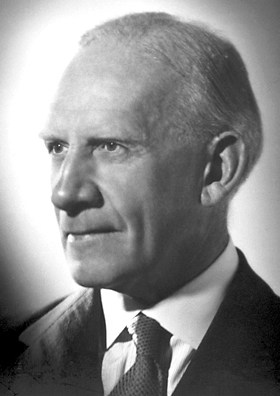
\includegraphics[width=\linewidth]{images/book3/robinson.jpg}
\end{minipage}\hfill
\begin{minipage}[t]{0.78\linewidth}
\vspace{0pt}
Robert Robinson et William Rapson publièrent cette séquence de formation de cycle en 1935, dans des
travaux visant la synthèse des stéroïdes. Les principales réussites de Robinson furent les structures
et les synthèses d'alcaloïdes, qui lui valurent le prix Nobel de chimie 1947. En 1950, Peter Wieland et
Karl Miescher préparèrent la dicétone bicyclique du problème de ce chapitre, devenue un point de départ
courant des synthèses de stéroïdes et de terpènes. (Portrait~: auteur inconnu, domaine public~;
Wikimedia Commons.)
\end{minipage}
\end{history}

\begin{safety}{\ghs[5mm]{GHS02}\,\ghs[5mm]{GHS05}\,\ghs[5mm]{GHS06}\,\ghs[5mm]{GHS07}\,\ghs[5mm]{GHS08}\,\ghs[5mm]{GHS09}}
La but-3-én-2-one est inflammable, très toxique, corrosive, dangereuse pour le milieu aquatique, et
fortement lacrymogène~; on ne la manipule que sous hotte. La cyclohex-2-én-1-one est inflammable et
toxique. Les organolithiens, les organomagnésiens et les cuprates réagissent violemment avec l'eau et
se manipulent sous gaz inerte.
% ledger: ghs:MVK, ghs:cyclohexenone, ghs:MeMgBr
\end{safety}

\section{Exercices}

\begin{exercise}[$\star$]\label{exo:b2:conjugate-additions:1}
Prévoir une \omterm{def:b2:conjugate-additions:addition-modes}{addition 1,2} ou 1,4 sur la cyclohex-2-én-1-one pour~: \ce{CH3MgBr}~; \ce{(CH3)2CuLi}~;
\ce{C6H5SH} avec un peu de base~; \ce{LiAlH4}.
\end{exercise}

\begin{exercise}[$\star$]\label{exo:b2:conjugate-additions:2}
Classer en donneur ou \omterm{def:b2:conjugate-additions:michael}{accepteur de Michael}~: la pentane-2,4-dione, le propènenitrile \ce{CH2=CHCN},
le nitrométhane, le propénoate de méthyle, le propanedioate de diéthyle, la but-3-én-2-one.
\end{exercise}

\begin{exercise}[$\star$]\label{exo:b2:conjugate-additions:3}
Écrire la préparation du dibutylcuprate de lithium à partir du 1-bromobutane, du lithium et de l'iodure de cuivre(I).
\end{exercise}

\begin{exercise}[$\star$]\label{exo:b2:conjugate-additions:4}
Donner le produit du propanedioate de diéthyle avec la but-3-én-2-one et une quantité catalytique
d'éthanolate de sodium, puis le produit obtenu après hydrolyse et chauffage.
\end{exercise}

\begin{exercise}[$\star\star$]\label{exo:b2:conjugate-additions:5}
Proposer une préparation de la 3-méthylcyclohexanone à partir de la cyclohex-2-én-1-one, et expliquer
pourquoi le bromure de méthylmagnésium serait un mauvais choix.
\end{exercise}

\begin{exercise}[$\star\star$]\label{exo:b2:conjugate-additions:6}
L'éthanethiol s'additionne sur la but-3-én-2-one en présence d'une trace de triéthylamine. Écrire le
mécanisme et dire pourquoi le thiolate s'additionne en 1,4.
\end{exercise}

\begin{exercise}[$\star\star$]\label{exo:b2:conjugate-additions:7}
Le cyanure donne avec la cyclohex-2-én-1-one, à basse température et pour des durées courtes, la
cyanhydrine~; à plus haute température et pour des durées plus longues, le
3-oxocyclohexane-1-carbonitrile. Expliquer à l'aide des contrôles cinétique et thermodynamique.
\end{exercise}

\begin{exercise}[$\star\star$]\label{exo:b2:conjugate-additions:8}
Donner le produit de l'\omterm{def:b2:conjugate-additions:robinson}{annélation de Robinson} de la 2-méthylcyclohexane-1,3-dione avec la
but-3-én-2-one, puis celui de la cyclohexanone avec la but-3-én-2-one.
\end{exercise}

\begin{exercise}[$\star\star$]\label{exo:b2:conjugate-additions:9}
Déconnecter l'heptane-2,6-dione en un donneur et un \omterm{def:b2:conjugate-additions:michael}{accepteur de Michael}, et proposer des conditions.
\end{exercise}

\begin{exercise}[$\star\star\star$]\label{exo:b2:conjugate-additions:10}
Une \omterm{def:b2:enolates-aldol:aldol}{aldolisation} simple est facilement renversée en milieu basique~; l'adduit de Michael du
propanedioate de diéthyle et de la but-3-én-2-one ne l'est pas. Expliquer à l'aide des liaisons
formées et rompues et de l'acidité du produit.
\end{exercise}

\begin{exercise}[$\star\star\star$]\label{exo:b2:conjugate-additions:11}
Le propanedioate de diéthyle avec deux équivalents de propénoate de méthyle et une base en quantité
catalytique donne un produit qui ne porte plus de liaison \ce{C-H} entre ses deux groupes ester. Le
représenter et expliquer.
\end{exercise}

\begin{exercise}[$\star\star\star$]\label{exo:b2:conjugate-additions:12}
Dans une \omterm{def:b2:conjugate-additions:robinson}{annélation de Robinson}, la 2-méthylcyclohexanone et la but-3-én-2-one peuvent réagir par
l'un ou l'autre \omterm{def:b2:enolates-aldol:enolate}{énolate}. Représenter les deux produits et dire quelles conditions favorisent celui qui
porte le groupe méthyle sur le carbone de jonction des cycles.
\end{exercise}

\section{Problème~: la cétone de Wieland--Miescher}

\begin{problem}[{Problème du week-end --- le donneur acide, l'adduit de Michael, l'aldolisation
intramoléculaire et sa déshydratation, le stéréocentre et le bilan de matière d'une préparation}]
\label{pb:b2:conjugate-additions:1}
Préparation (données de l'exercice)~: \qty{10.0}{g} de 2-méthylcyclohexane-1,3-dione réagissent avec
un léger excès de but-3-én-2-one et une base en quantité catalytique (\omterm{def:b2:conjugate-additions:michael}{addition de Michael})~; la
tricétone est ensuite cyclisée par une \omterm{def:b2:amines:class}{amine secondaire} et un acide (\omterm{def:b2:enolates-aldol:aldol}{aldolisation}, déshydratation).
Rendement global~: 70~\%. La cyclohexane-1,3-dione parente a un
$\mathrm pK_a = 5.3$ dans l'eau. Masses molaires (\unit{g/mol})~: C 12.011, H 1.008, O 15.999.
% ledger: pka:cyclohexanedione, aw:C, aw:H, aw:O, ghs:methylcyclohexanedione, ghs:MVK

\medskip
\noindent\textbf{Partie I --- Le donneur.}
\begin{enumerate}
  \item Représenter la 2-méthylcyclohexane-1,3-dione et repérer son hydrogène le plus acide.
  \item Pourquoi cet hydrogène est-il tellement plus acide que les hydrogènes $\alpha$ de la cyclohexanone~?
  \item Représenter les trois formes mésomères de son \omterm{def:b2:enolates-aldol:enolate}{énolate}.
  \item L'hydroxyde ou l'éthanolate est-il assez fort pour former totalement cet \omterm{def:b2:enolates-aldol:enolate}{énolate}~? Utiliser le $\mathrm pK_a$.
  \item Écrire l'\omterm{def:b2:enolates-aldol:tautomerism}{énol} de la dione qui fait intervenir C2, et dire pourquoi le groupe méthyle porté par C2
        ne l'empêche pas.
  \item Cet \omterm{def:b2:enolates-aldol:enolate}{énolate} est-il dur ou mou~? Quel site de la but-3-én-2-one attaquera-t-il~?
\end{enumerate}

\medskip
\noindent\textbf{Partie II --- L'adduit de Michael.}
\begin{enumerate}[resume]
  \item Écrire l'\omterm{def:b2:conjugate-additions:michael}{addition de Michael} et nommer la tricétone formée.
  \item Pourquoi une quantité catalytique de base suffit-elle~?
  \item Pourquoi la nouvelle liaison se forme-t-elle sur le C2 de la dione plutôt que sur son oxygène~?
  \item Combien la tricétone possède-t-elle de carbones quaternaires~?
  \item Repérer la relation 1,5-dicarbonylée dans la tricétone.
  \item Pourquoi utilise-t-on un léger excès de but-3-én-2-one, et pourquoi seulement léger~?
\end{enumerate}

\medskip
\noindent\textbf{Partie III --- La fermeture du cycle.}
\begin{enumerate}[resume]
  \item Énumérer les carbones de la tricétone qui portent des hydrogènes $\alpha$.
  \item Quel \omterm{def:b2:enolates-aldol:enolate}{énolate}, attaquant quel carbonyle, ferme un cycle à six atomes~?
  \item Quelles autres fermetures de cycle pourrait-on envisager, et pourquoi ne donnent-elles pas le produit~?
  \item Écrire l'\omterm{def:b2:enolates-aldol:aldol}{aldol} formé et la déshydratation qui suit.
  \item Pourquoi la déshydratation est-elle facile~?
  \item Nommer les groupes fonctionnels de la cétone de Wieland--Miescher.
\end{enumerate}

\medskip
\noindent\textbf{Partie IV --- Stéréochimie et bilan de matière.}
\begin{enumerate}[resume]
  \item Quel carbone du produit est un stéréocentre~?
  \item Le produit de cette préparation est-il optiquement actif~? Expliquer.
  \item Calculer les masses molaires de la dione, de la but-3-én-2-one et du produit
        \ce{C11H14O2}.
  \item Écrire l'équation globale et la vérifier à l'aide des formules.
  \item Calculer la quantité de dione utilisée.
  \item Donner la masse de cétone de Wieland--Miescher obtenue avec un rendement global de 70~\%.
\end{enumerate}
\end{problem}
